\documentclass[12pt,ucs,hyperref={pdftext}]{beamer}
%\documentclass[12pt, a4paper]{article}
\mode<presentation>

\newif\ifpdf
\ifx\pdfoutput\undefined
\pdffalse % we are not running PDFLaTeX
\else
\pdfoutput=1 % we are running PDFLaTeX
\pdftrue
\fi
%\usetheme{Warsaw}
%\usetheme{Berkeley}
%\usetheme{PaloAlto}
\usetheme{Luebeck}
\usecolortheme[]{seagull}
%\usecolortheme[]{beaver}

%\usepackage{mathptmx}
%\usepackage{helvet}

\usepackage[utf8x]{inputenc}
\usepackage[english]{babel}
%\usepackage{german}
%\usepackage{longtable}
%\usepackage{tocbibind}
%\usepackage{makeidx}
%\usepackage{amsmath}
%\usepackage{amsfonts}
%\usepackage{amssymb}
%\usepackage{pdfsync}  % enable tex source and pdf output syncronicity
%\usepackage[all]{xy}
\usepackage{multicol}
%\usepackage{wrapfig}
\usepackage{listings}

\lstset{
	language=C++,
	basicstyle=\ttfamily\small, % print whole listing small
	keywordstyle=\color{blue},%\bfseries,
	identifierstyle=, % nothing happens
	commentstyle=\color{green}, % white comments
	stringstyle=\color{red}\ttfamily, % typewriter type for strings
	showstringspaces=false,
	numbers=left, numberstyle=\tiny, stepnumber=1, numbersep=5pt,
	columns=flexible,% fixed
	breaklines=true,
	tabsize=4,
	xleftmargin=1em
}

\lstdefinelanguage{lua}
{
	morecomment = [l]{--},
	morecomment = [s]{--[[}{]]}, % lua supports more
	morestring=[b]",
	morestring=[b]',
	sensitive = true,
	morekeywords = {
	and, break, do, else, elseif,
	end, false, for, function, if,
	in, local, nil, not, or, repeat,
	return, then, true, until, while }
}

\hypersetup{
    pdftitle={Designing and implementing a flexible and extensible testing framework},
%    pdfsubject={Subject of the document}, % Subject
    pdfauthor={Gerhard Roethlin},              % Author
    pdfkeywords={master, fatigue testing software, stereo vision},       % Keywords
}

\setbeamertemplate{navigation symbols}{\insertframenavigationsymbol}

%\renewcommand{\labelitemi}{-}

\setcounter{tocdepth}{2}

\setbeamercovered{transparent=25}
\setbeamersize{description width=0.5cm}
\newlength{\columnleft}
\newlength{\columnright}
\setlength{\columnleft}{5cm}
\setlength{\columnright}{6cm}

%\titlegraphic{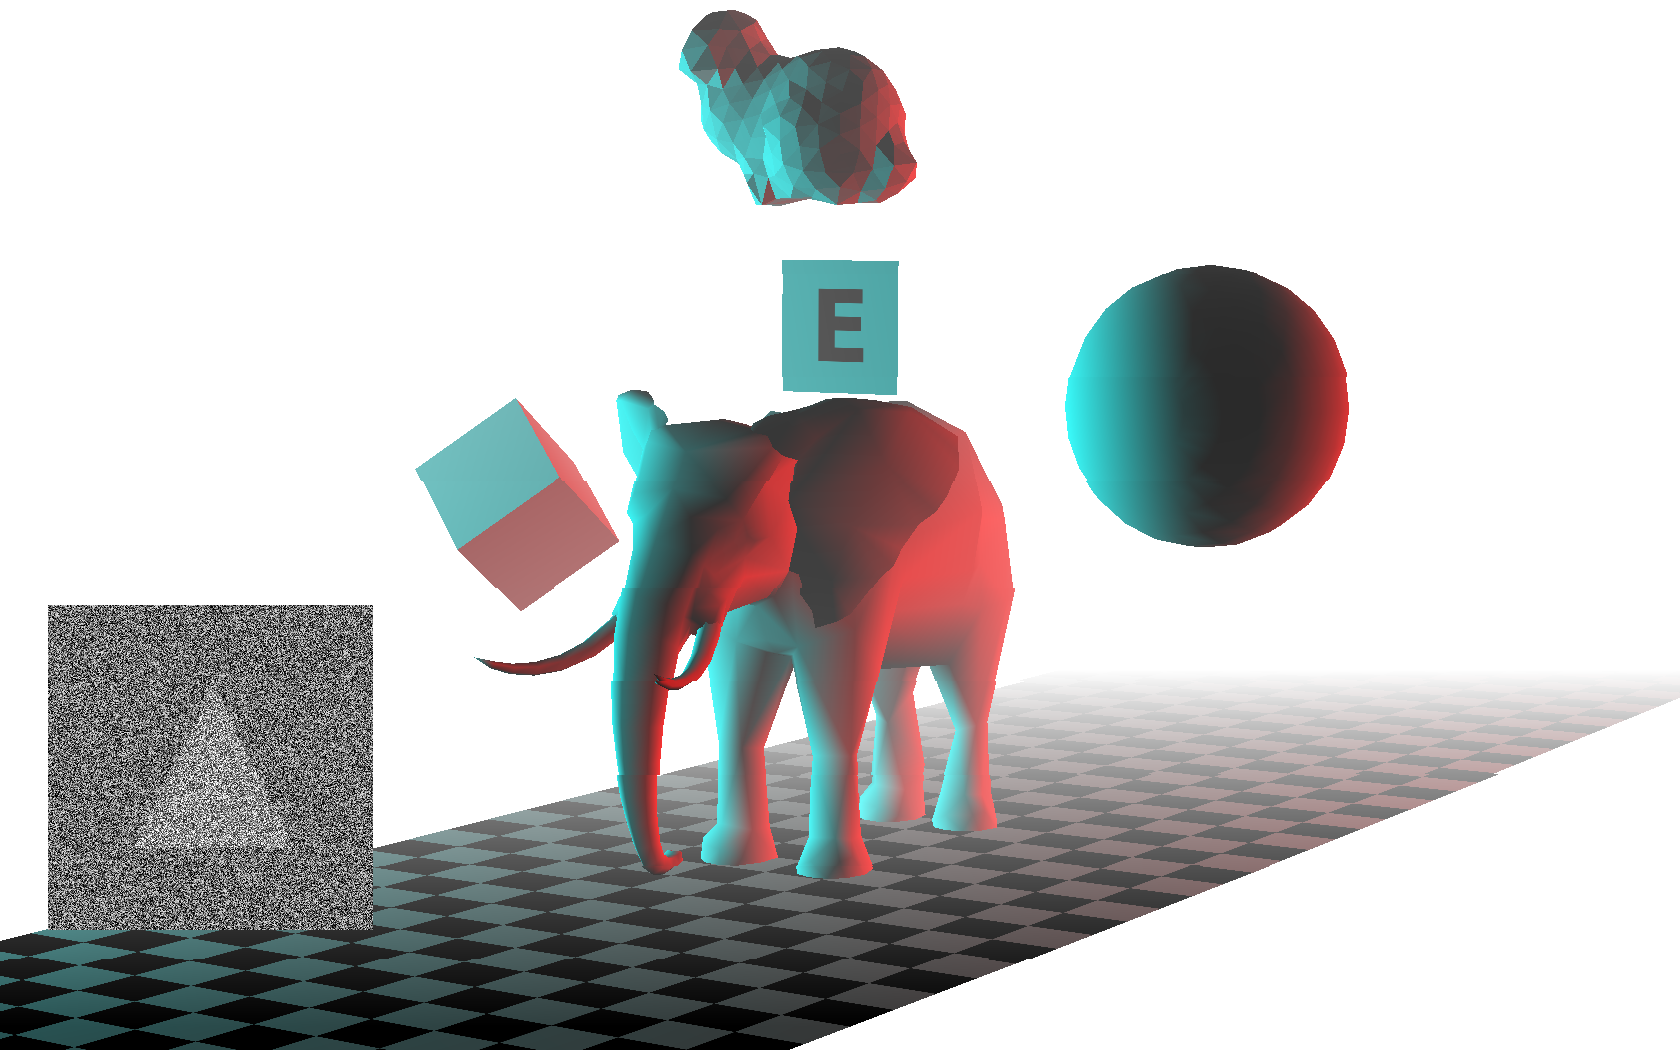
\includegraphics[width=7.5cm,clip,trim=0cm 6cm 0cm 2cm]{media/title.png}}
\title{ExaminationRoom}
\subtitle{Designing and implementing a flexible and extensible testing framework}
\author[gerhardr]{Gerhard R\"othlin {\tt\normalsize <cbreak@the-color-black.net>}}
\date{2008.07.07}

\begin{document}

\ifpdf
\DeclareGraphicsExtensions{.pdf, .jpg, .tif, .tiff, .png}
\else
\DeclareGraphicsExtensions{.eps, .jpg}
\fi

\begin{frame}

\titlepage
%\inserttitlegraphic
%\inserttitle
%\insertsubtitle
%\insertauthor
%\insertdate
%\insertinstitute

\end{frame}

%\logo{\includegraphics[width=1cm,alpha=0.5]{media/icon-mayan.png}}


\section{Introduction}

\subsection{Outline}

\begin{frame}{Outline}
\begin{multicols}{2}
\tableofcontents
\end{multicols}
\end{frame}


\subsection{Motivation}

\begin{frame}{Motivation}
\begin{columns}

\column{\columnleft}
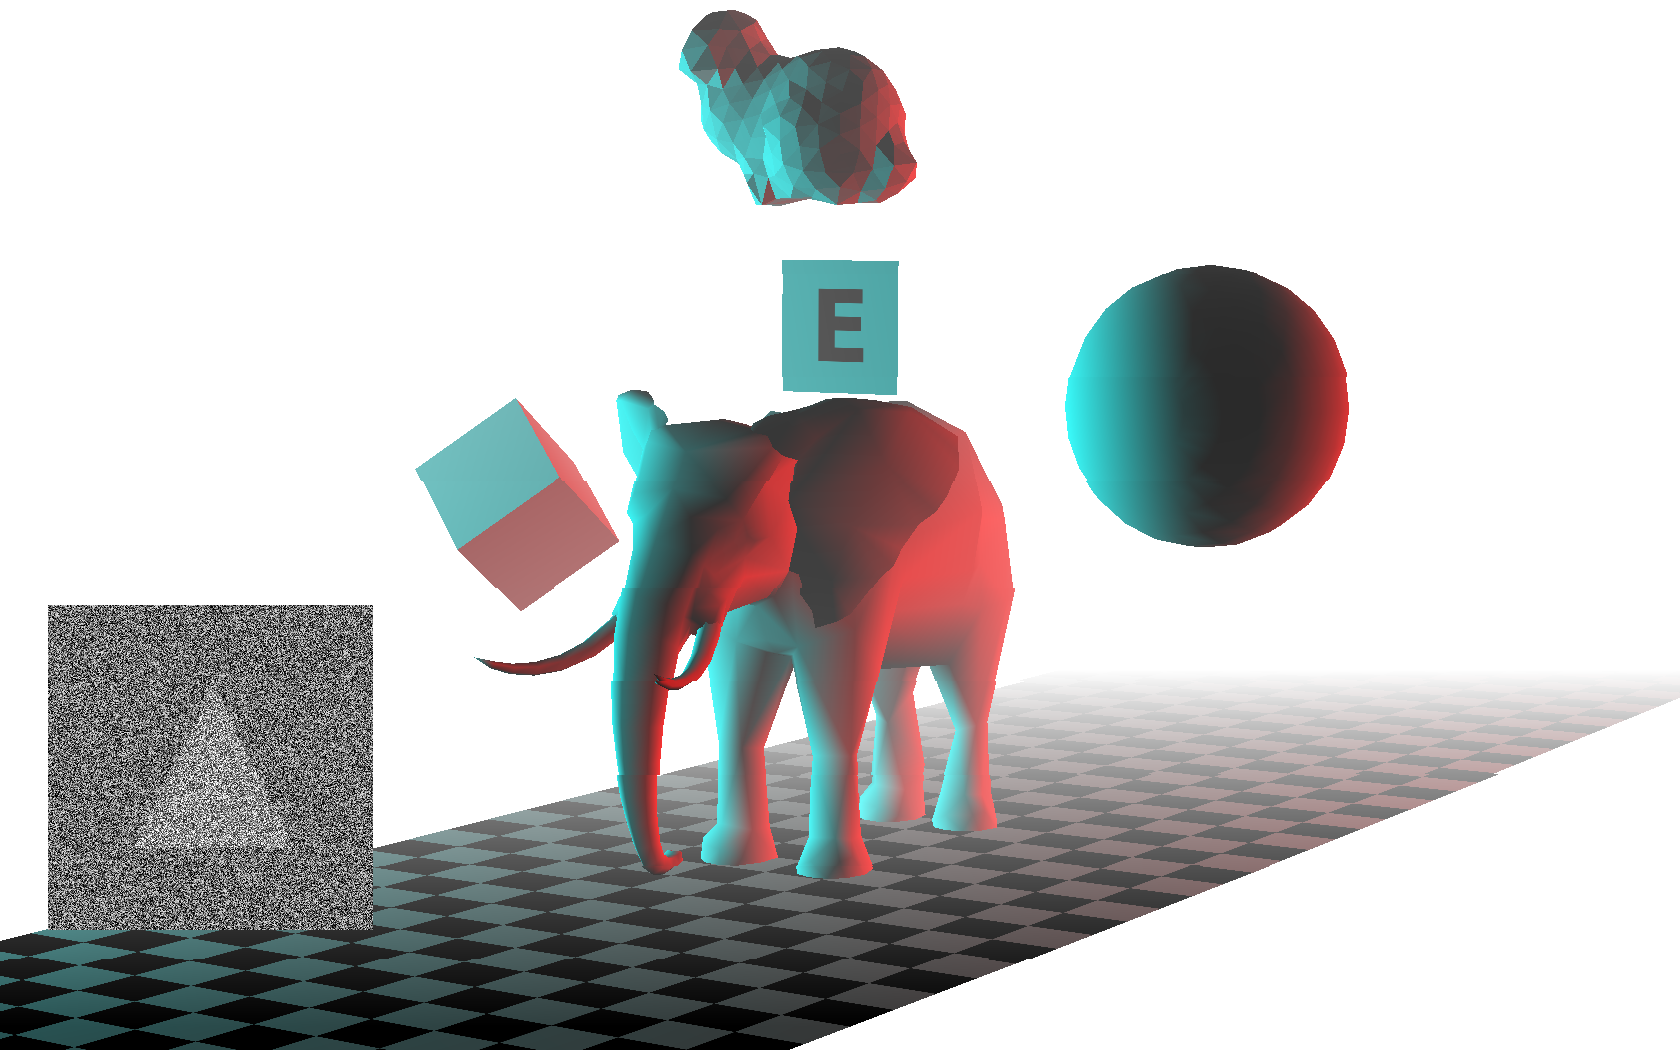
\includegraphics[width=\columnleft]{media/title.png}

\column{\columnright}
\begin{itemize}%[<+-| alert@+>]%[<+->]
\item Understanding how humans see stereo stimuli could improve stereo film making
\item Psychological tests are widely used to study human perception
\item The tools used for such tests are very restrictive in terms of stimuli and test design
\end{itemize}

\end{columns}
\end{frame}


\begin{frame}{Questions}
\begin{columns}

\column{\columnleft}
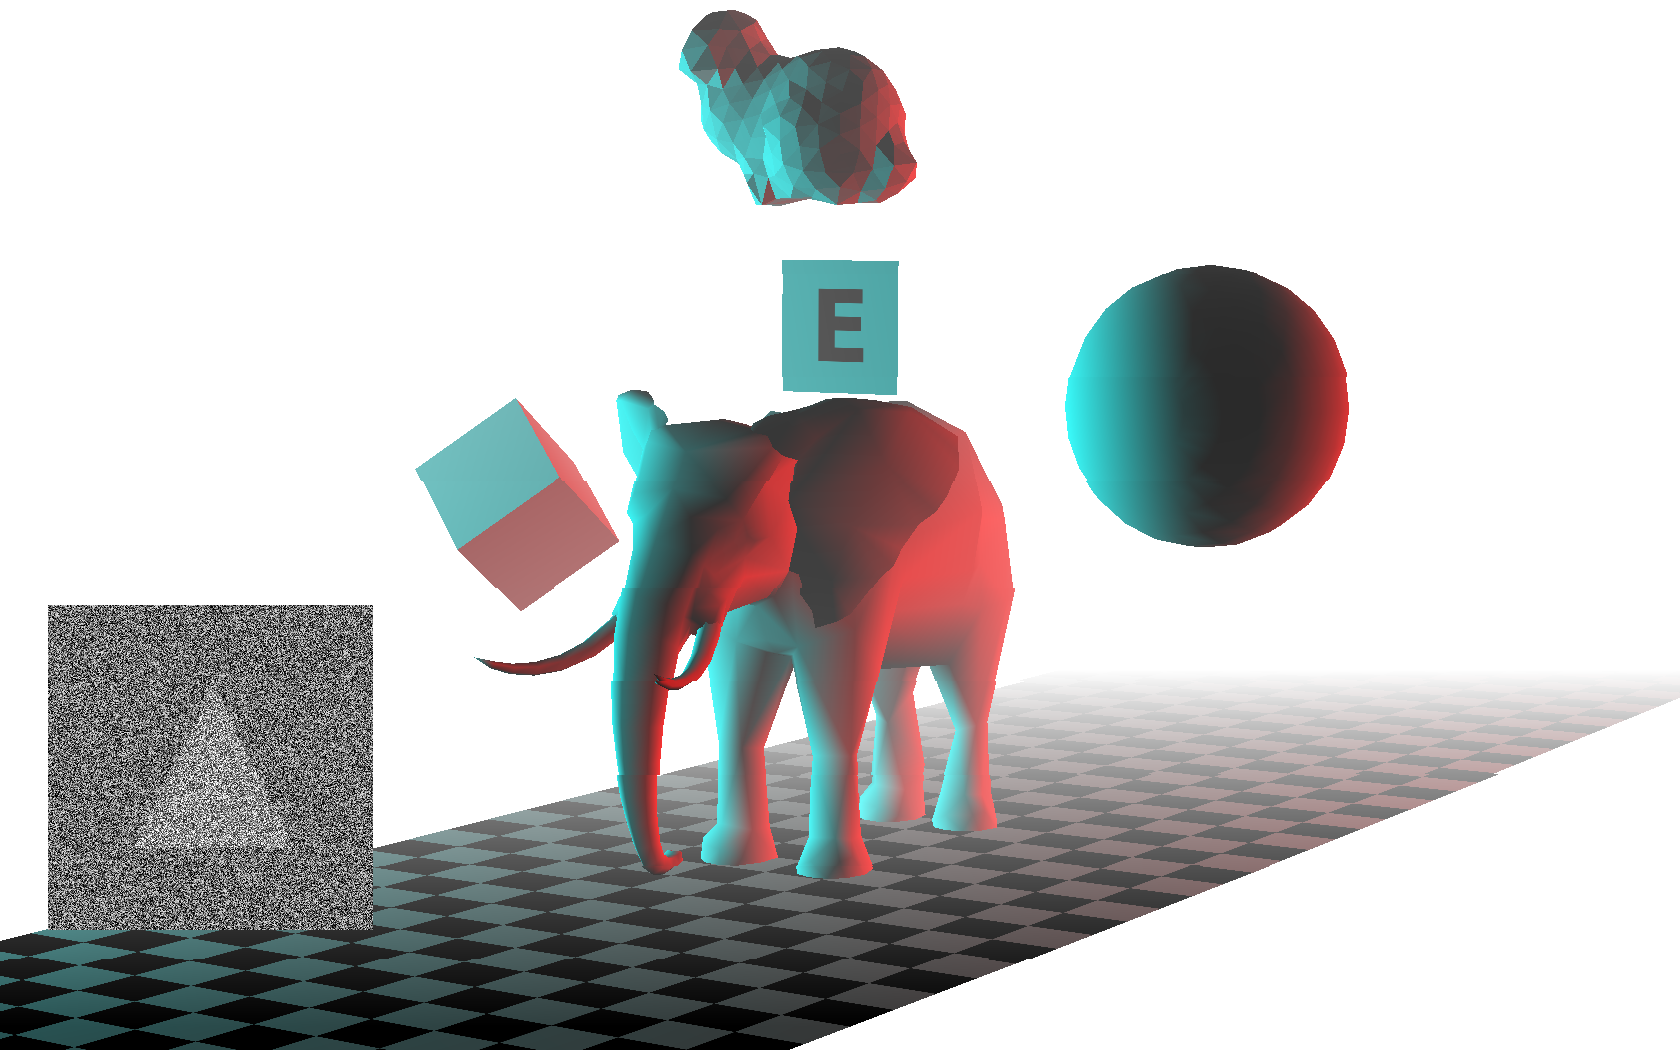
\includegraphics[width=\columnleft]{media/title.png}

\column{\columnright}
\begin{itemize}%[<+-| alert@+>]%[<+->]
\item Which features would simplify the creation and conduction of such tests?
\item How can a tool be flexible enough to support every imaginable test, while still be user friendly?
\item What is the right tradeoff between power and usability?
\end{itemize}

\end{columns}
\end{frame}


\section{Design}

\begin{frame}{Design}
\begin{columns}

\column{\columnleft}

\column{\columnright}
\begin{itemize}%[<+-| alert@+>]%[<+->]
\item TODO: Design is
\item Requirement: Cues
\item Requirement: Usability (GUI)
\end{itemize}

\end{columns}
\end{frame}

\subsection{Cues}

\begin{frame}{Cues}
\begin{columns}

\column{5.5cm}
\begin{itemize}
\item<uncover@0> Projection
\begin{itemize}
\item Relative Size/Density
\item Motion Perspective
\item Convergence (proprioception)
\item Binocular Stereopsis
\end{itemize}

\item<uncover@0> Physical
\begin{itemize}
\item Occlusion
\item Aerial Perspective
\item Light \& Shading
\item Accommodation
\end{itemize}

\end{itemize}

\column{5.5cm}
\begin{itemize}%[<+-| alert@+>]%[<+->]
\item Depth Cues help perceiving depth
\item They differ in their cause and the way they are perceived
\item For testing it would be nice to be able to turn them on and off at will
\end{itemize}

\end{columns}
\end{frame}

\begin{frame}{Projection Cues}
\begin{columns}

\column{5.5cm}
\begin{itemize}
\item Projection
\begin{itemize}
\item Relative Size/Density
\item Motion Perspective
\item Convergence (proprioception)
\item Binocular Stereopsis
\end{itemize}

\item<uncover@0> Physical
\begin{itemize}
\item Occlusion
\item Aerial Perspective
\item Light \& Shading
\item Accommodation
\end{itemize}

\end{itemize}

\column{5.5cm}
\begin{itemize}%[<+-| alert@+>]%[<+->]
\item Projection is transformation of 3D to 2D space
\item Humans perform this projection physically with the eye
\item Projection cues are closely related, they can not easily be eliminated selectively
\item Camera nodes allow mixing of different projection
\end{itemize}

\end{columns}
\end{frame}

\begin{frame}{Physical Cues}
\begin{columns}

\column{5.5cm}
\begin{itemize}
\item<uncover@0> Projection
\begin{itemize}
\item Relative Size/Density
\item Motion Perspective
\item Convergence (proprioception)
\item Binocular Stereopsis
\end{itemize}

\item Physical
\begin{itemize}
\item Occlusion
\item Aerial Perspective
\item Light \& Shading
\item Accommodation
\end{itemize}

\end{itemize}

\column{5.5cm}
\begin{itemize}%[<+-| alert@+>]%[<+->]
\item Physical cues are created by the properties of the world
\item They can often be added or removed by changing drawing code
\item Accommodation changes require physical modification
\end{itemize}

\end{columns}
\end{frame}



\subsection{Scene graph}

\begin{frame}{Scene Graph}
\begin{columns}

\column{\columnleft}
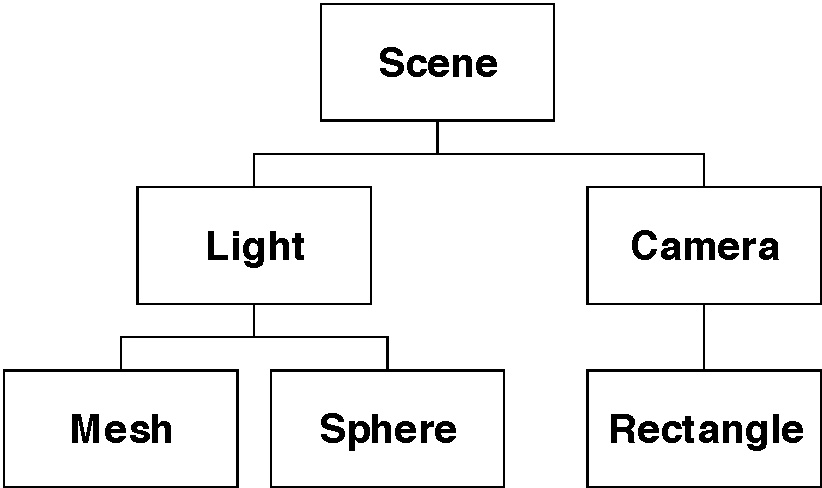
\includegraphics[width=\columnleft]{media/scene.pdf}

\column{\columnright}
\begin{itemize}%[<+-| alert@+>]%[<+->]
\item A scene-graph organizes objects in a scene
\item The graph in this app is state sorted, state applies to all children
\item An alternative would be spatial sorting
\item State sorting speeds up drawing and simplifies implementation of many special effects
\end{itemize}

\end{columns}
\end{frame}


\subsection{User Interface}

\begin{frame}{Creation}
\begin{columns}

\column{\columnleft}

\column{\columnright}
\begin{itemize}%[<+-| alert@+>]%[<+->]
\item TODO: Explain how scenes are created in the UI
\item State how it simplifies creation
\end{itemize}

\end{columns}
\end{frame}


\section{Implementation}


\subsection{Frameworks}

\begin{frame}{Frameworks}
\begin{columns}

\column{\columnleft}

\begin{center}

\includegraphics[width=2cm]{media/logo/qt_original_r.pdf}

\bigskip


\includegraphics[width=2cm]{media/logo/lua-logo-label.pdf}

\bigskip


\includegraphics[width=4cm]{media/logo/boost-vec-white.pdf}
\end{center}

\column{\columnright}
\begin{itemize}%[<+-| alert@+>]%[<+->]
\item Qt: Cross platform UI and Core API from \textit{Trolltech}
\item Boost: Header library that extends \textit{C++}'s \lstinline{std::}
\item Lua: Embedded scripting language
\item LuaBridge: Binding library
\item OpenGL: 3D drawing library
\item libobj: obj mesh loader library
\end{itemize}

\end{columns}
\end{frame}


\subsection{Interesting Code}

\begin{frame}{Object}
\begin{columns}

\column{\columnleft}

\begin{center}
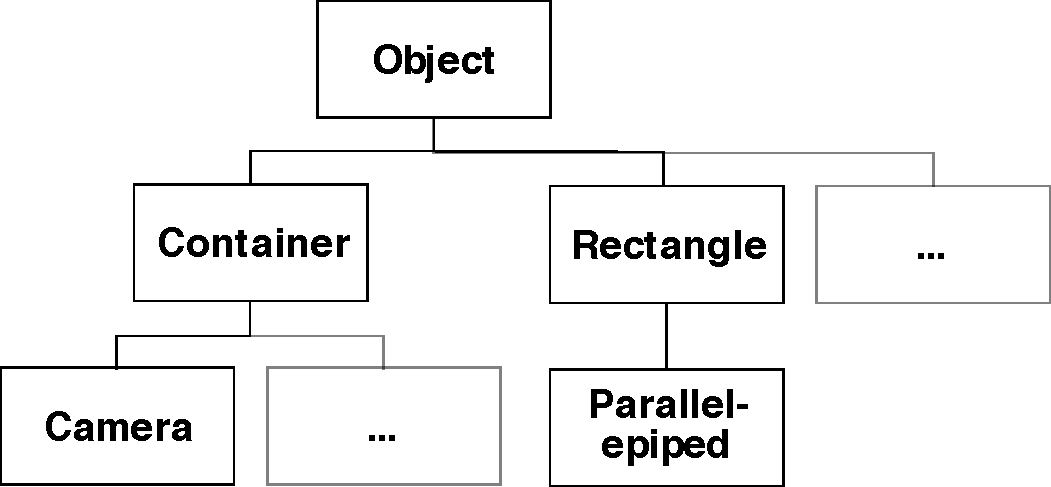
\includegraphics[width= \columnleft]{media/object.pdf}
\end{center}

\column{\columnright}
\begin{itemize}%[<+-| alert@+>]%[<+->]
\item Object is the parent class of everything in the scene-graph
\item An object is usually something that is drawable
\item An object can have an associated texture, color, position and other parameters
\item A dialog box can be used to change those parameters
\item An object can serialize itself
\end{itemize}

\end{columns}
\end{frame}

\begin{frame}{Objects}
\begin{columns}

\column{\columnleft}

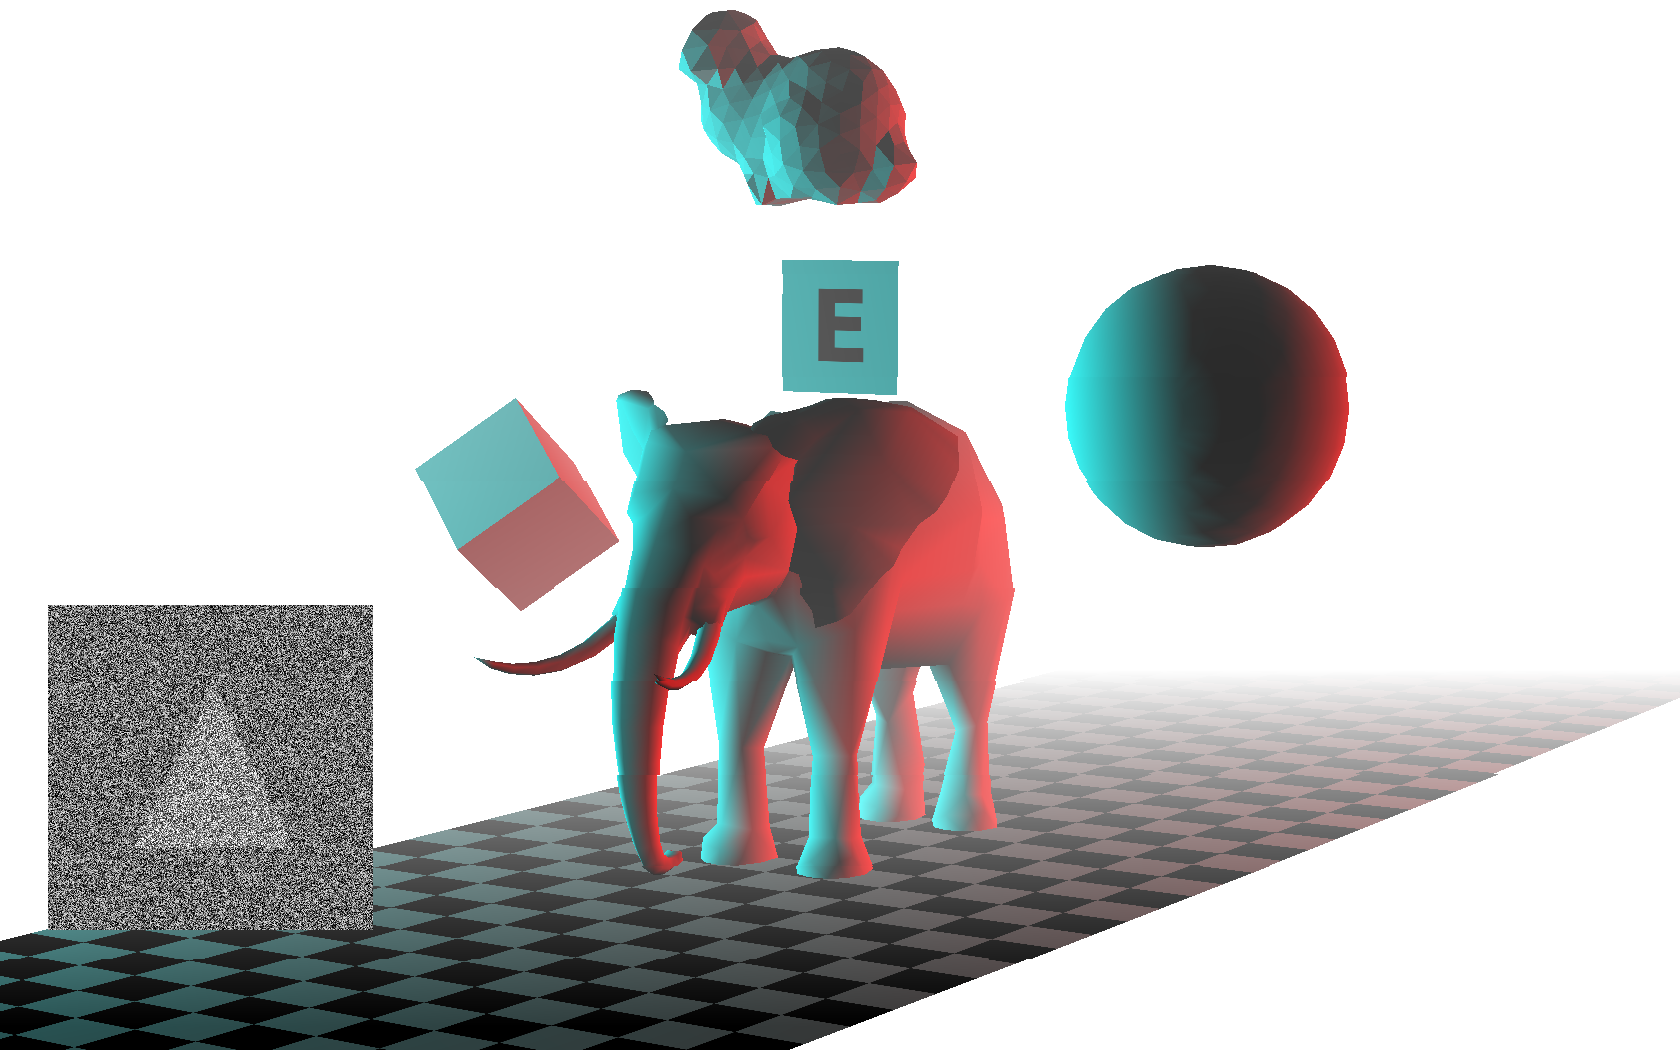
\includegraphics[width=\columnleft]{media/title.png}

\column{\columnright}
\begin{itemize}%[<+-| alert@+>]%[<+->]
\item Primitive objects
\begin{itemize}
\item Rectangle
\item Parallelepiped
\item Sphere
\end{itemize}
\item Pixelplane
\item Mesh
\item Text
\item Container
\end{itemize}

\end{columns}
\end{frame}

\begin{frame}{Container Nodes}
\begin{columns}

\column{\columnleft}
\begin{itemize}
\item AffineTransformation
\item Atmosphere
\item CameraNode
\item DepthBuffer
\item LightNode
\item ...
\end{itemize}

\column{\columnright}
\begin{itemize}%[<+-| alert@+>]%[<+->]
\item TODO: Describe Container Nodes
\end{itemize}

\end{columns}
\end{frame}


\begin{frame}{Camera}
\begin{columns}

\column{\columnleft}

\begin{center}
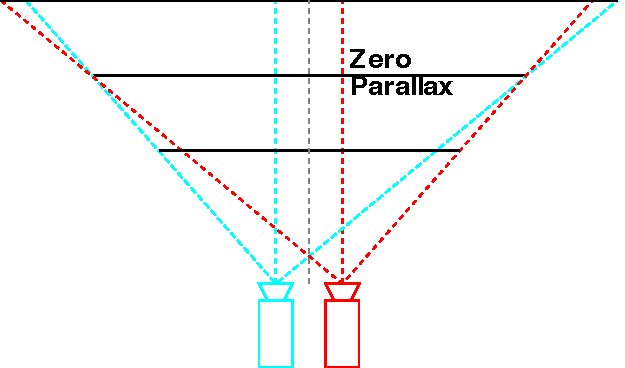
\includegraphics[width=4.5cm]{media/camera-perspective.pdf}

\bigskip

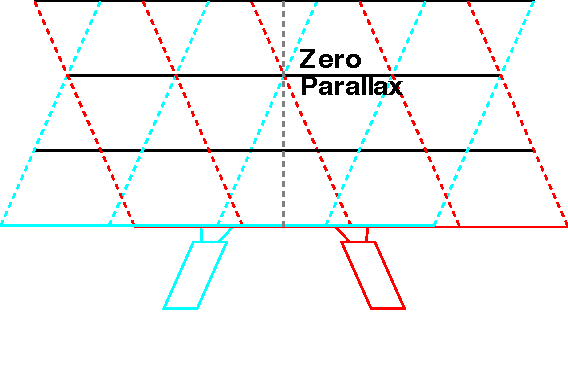
\includegraphics[width=4.5cm]{media/camera-parallel.pdf}
\end{center}

\column{\columnright}
\begin{itemize}%[<+-| alert@+>]%[<+->]
\item TODO
\end{itemize}

\end{columns}
\end{frame}

\begin{frame}{Stereograms}
\begin{columns}

\column{\columnleft}
\begin{center}
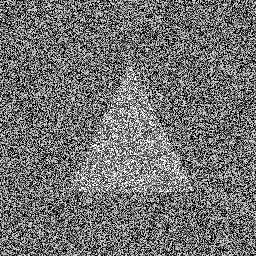
\includegraphics[scale=0.25]{screenshots/rds_example.png}

\bigskip

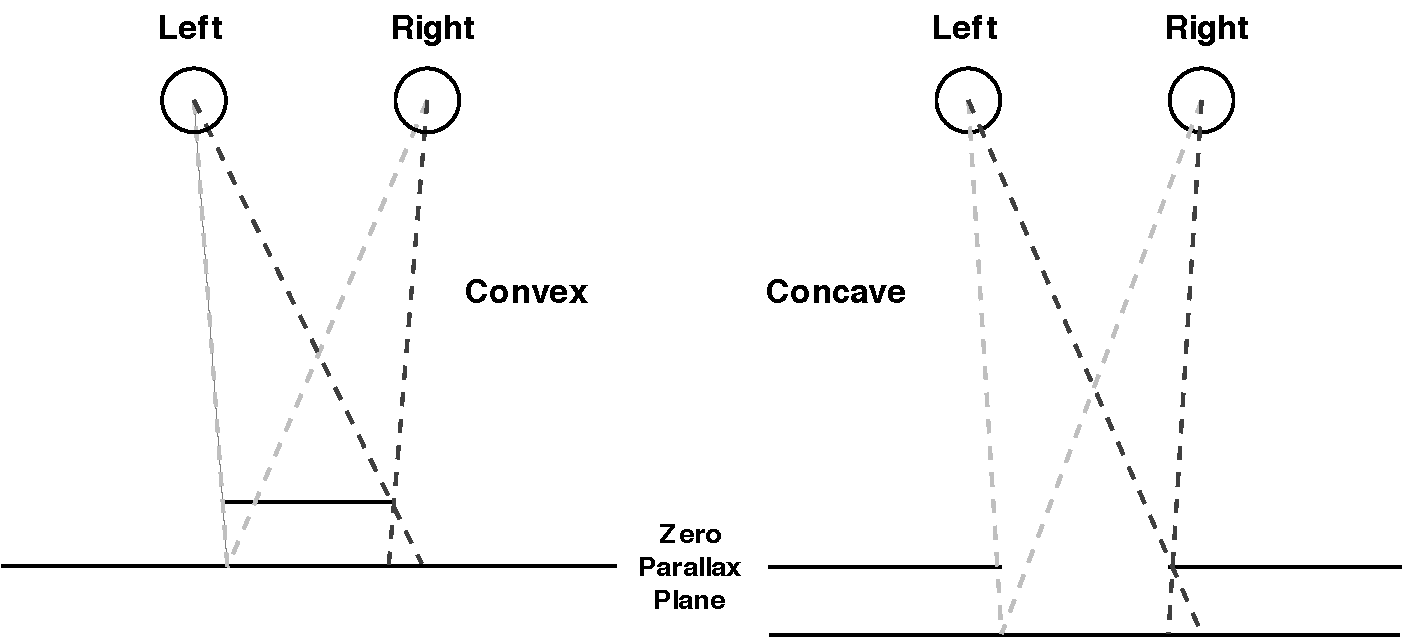
\includegraphics[scale=0.25]{media/rds.pdf}
\end{center}

\column{\columnright}
\begin{itemize}%[<+-| alert@+>]%[<+->]
\item Random dot stereogram encodes information so that it is mathematically impossible to see monoscopically
\item Custom algorithm creates random dot patterns with different colors for fg/bg
\item Slightly different algorithm for convex and concave
\end{itemize}

\end{columns}
\end{frame}


\subsection{Mechanics}

\begin{frame}{Lua}
\begin{columns}

\column{\columnleft}

\column{\columnright}
\begin{itemize}%[<+-| alert@+>]%[<+->]
\item TODO: Explain what lua is
\end{itemize}

\end{columns}
\end{frame}

\begin{frame}{Scene Format}
\begin{columns}

\column{\columnleft}

\begin{center}
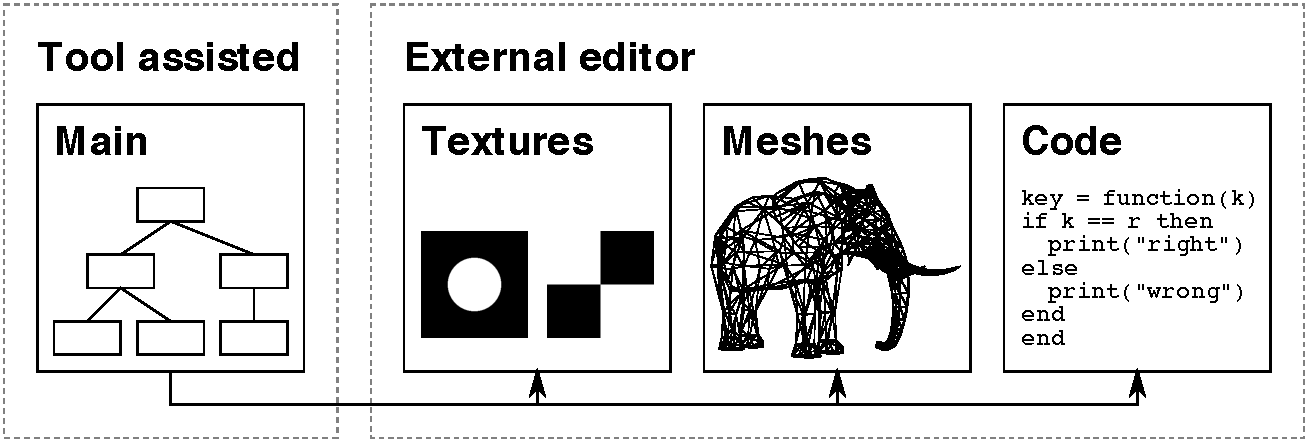
\includegraphics[width=5cm]{media/document.pdf}
\end{center}

\column{\columnright}
\begin{itemize}%[<+-| alert@+>]%[<+->]
\item TODO: Describe scene format
\end{itemize}

\end{columns}
\end{frame}

\begin{frame}{Example}
\begin{columns}

\column{\columnleft}

\column{\columnright}
\begin{itemize}%[<+-| alert@+>]%[<+->]
\item TODO
\end{itemize}

\end{columns}
\end{frame}


\section{Conclusion}

\subsection{Demo}

\begin{frame}{Creation Demo}
A short demo of the test creation
\end{frame}

\begin{frame}{Test Demo}
A short demo of the testing
\end{frame}


\subsection{Final thoughts}

\begin{frame}{Final thoughts}
\begin{columns}

\column{\columnleft}
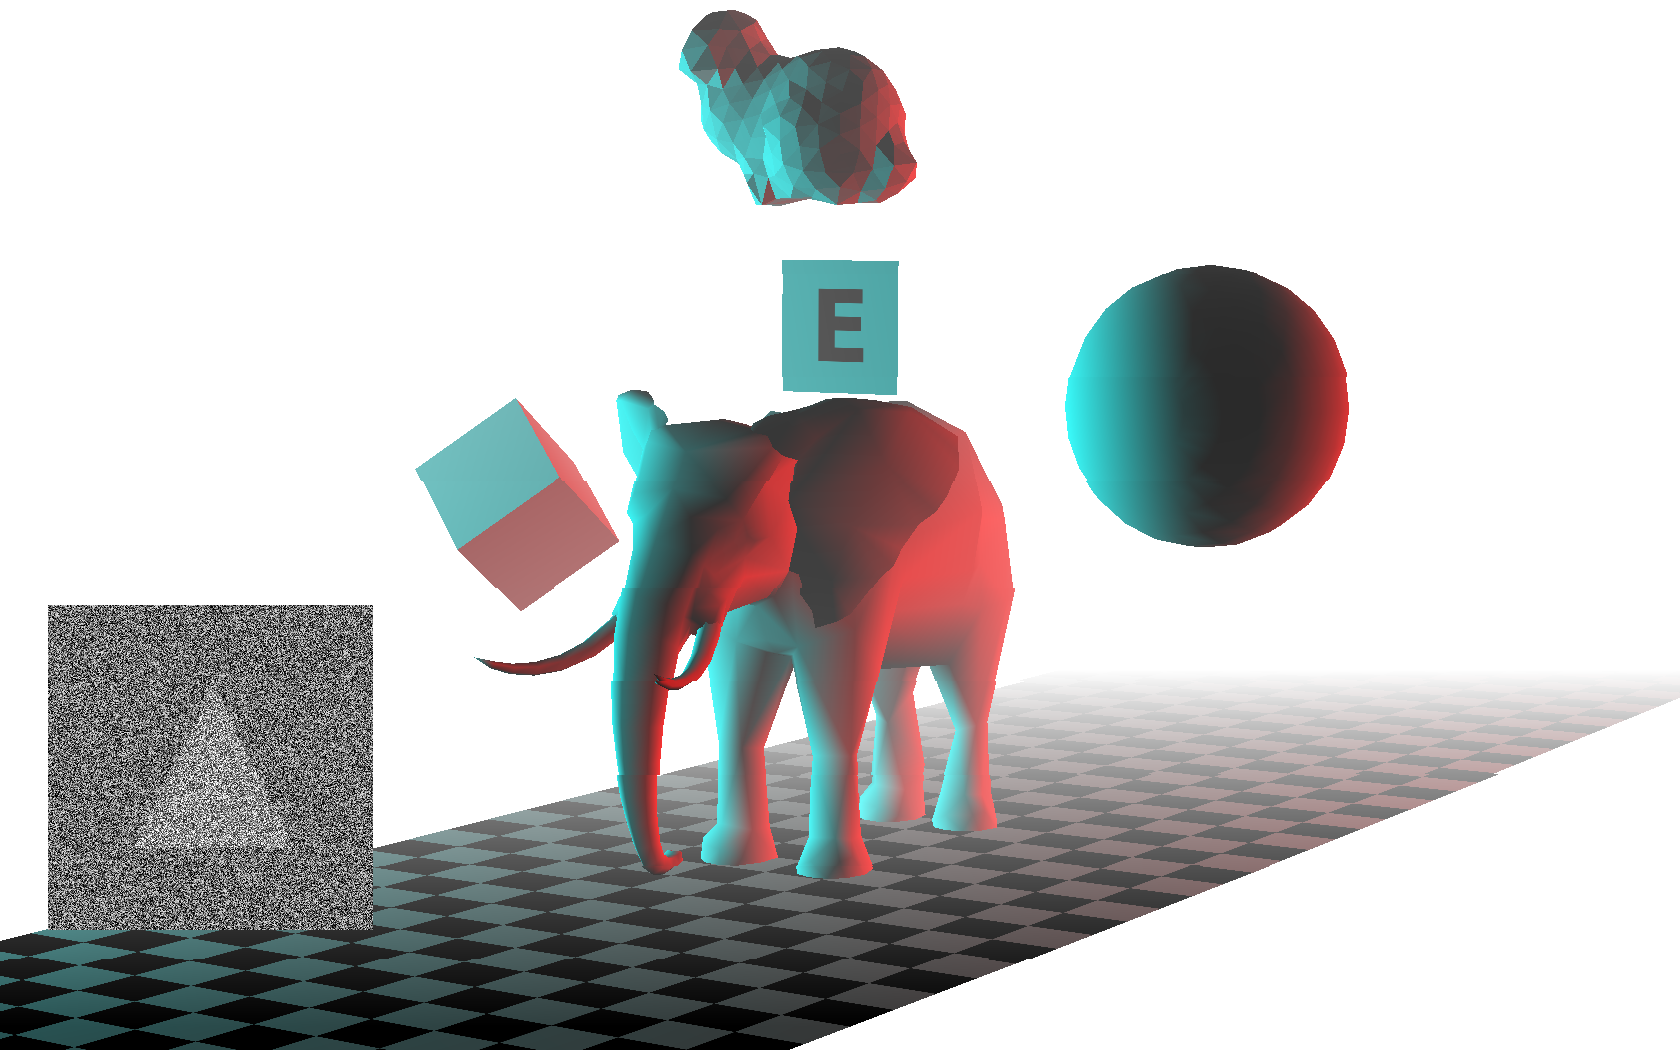
\includegraphics[width=\columnleft]{media/title.png}

\column{\columnright}
\begin{itemize}%[<+-| alert@+>]%[<+->]
\item Many of the features help with creation of the stimuli
\begin{itemize}
\item GUI for scene graph manipulation
\item Immediate feedback
\end{itemize}
\item Creating the mechanics of a test is hard
\begin{itemize}
\item Simplified by sacrificing flexibility.
\item Limit tests to a standard pattern with trials, blocks
\end{itemize}
\end{itemize}

\end{columns}
\end{frame}

\begin{frame}{Future}
\begin{columns}

\column{\columnleft}
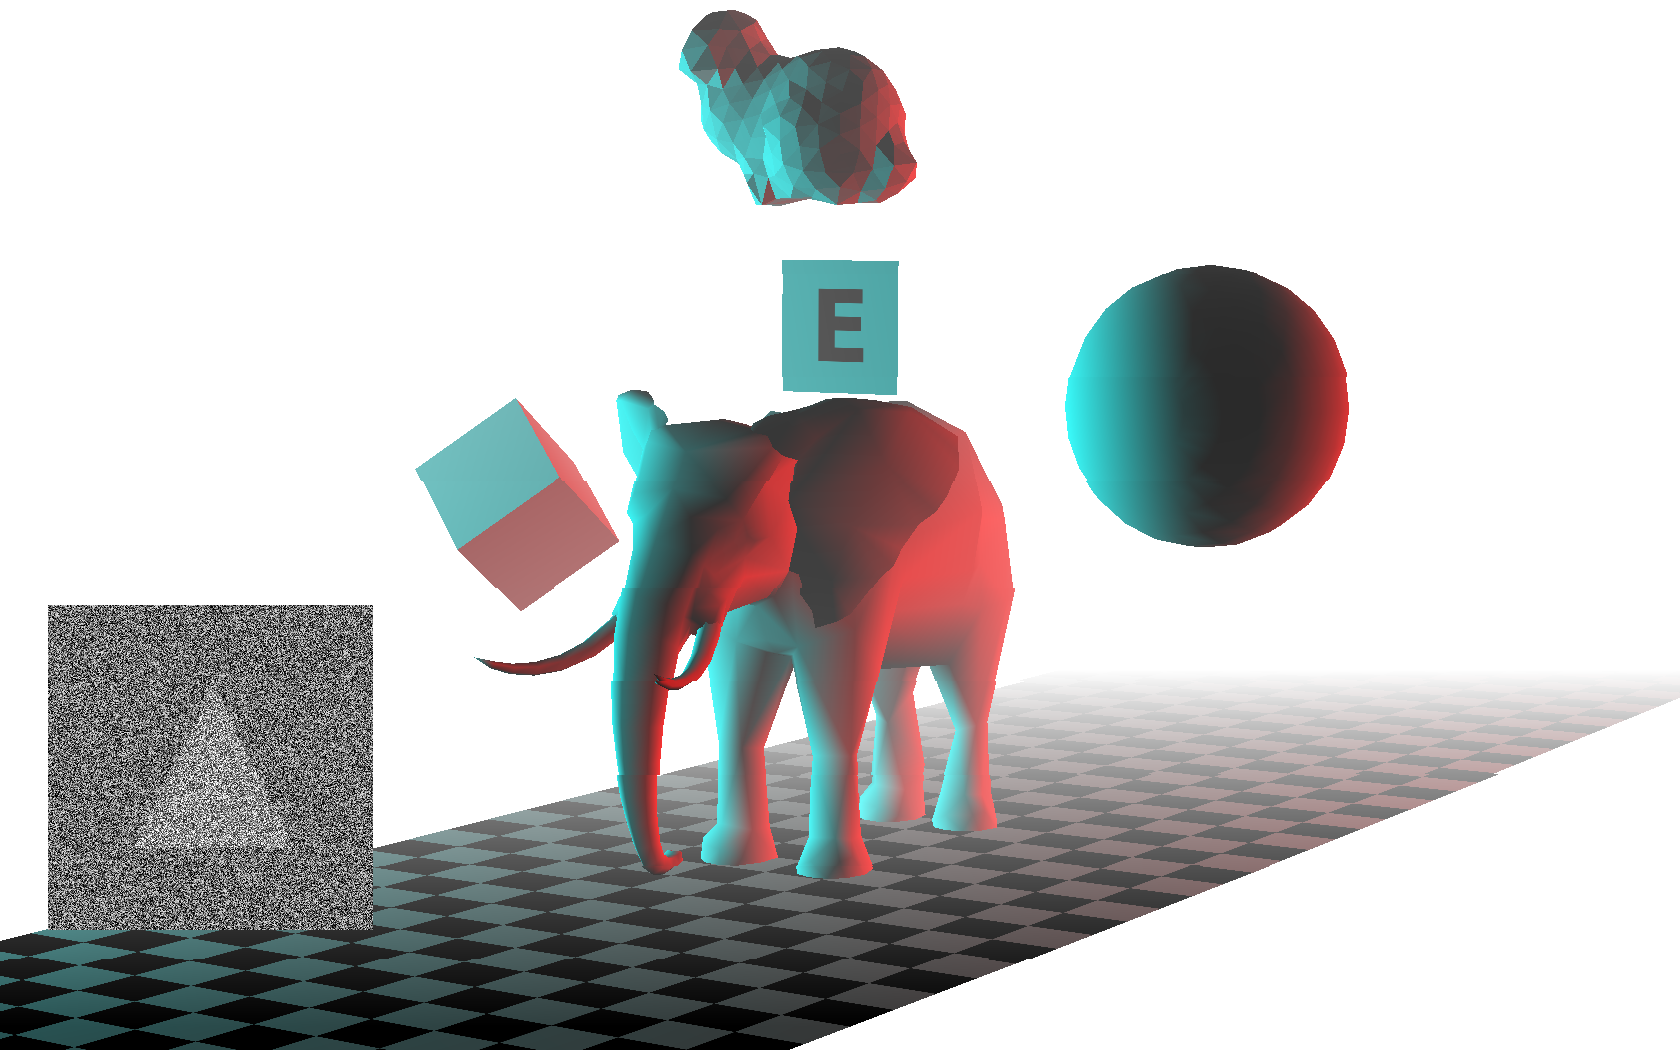
\includegraphics[width=\columnleft]{media/title.png}

\column{\columnright}
\begin{itemize}%[<+-| alert@+>]%[<+->]
\item Architectural changes for easier extensibility
\item User Interface changes for easier programmability
\end{itemize}

\end{columns}
\end{frame}


\appendix


\subsection{End?}
\begin{frame}{End}
Questions?
\end{frame}

\subsection{Examples}



\end{document}
\end
